\documentclass[aps,pra,twocolumn,reprint,floatfix,amsmath,amssymb]{revtex4-2}

\usepackage{graphicx}
\usepackage{booktabs}
\usepackage{siunitx}
\usepackage[colorlinks=true,linkcolor=blue,citecolor=blue,urlcolor=blue]{hyperref}
\usepackage{array}

\begin{document}

\title{\texorpdfstring{Shared-Line Multitone SQR in Dispersive cQED:\\
A Controlled No-Go, the Decoupled-Block Exception, and Only Partial Echo Relief}{Shared-Line Multitone SQR in Dispersive cQED: A Controlled No-Go, the Decoupled-Block Exception, and Only Partial Echo Relief}}
\author{Autonomous cQED Research Platform}
\affiliation{Shyam Shankar Quantum Circuits Group}
\date{\today}

\begin{abstract}
This study examines a deliberately narrow question: whether an ideal simultaneous selective qubit rotation can be realized exactly in dispersive circuit quantum electrodynamics when a shared qubit-control line carries one resonant tone per addressed cavity manifold, no artificial per-tone detuning is allowed, and the only free corrections are per-tone amplitude and azimuth. Several earlier local studies were suggestive but did not answer this exact question because they allowed frequency offsets or moved to richer waveform families. In the controlled block-resolved dispersive limit, a Magnus analysis shows that spectator tones generate blockwise effective \(Z\) terms. For the two-block square-pulse problem the second-order coefficients are explicit, and forcing both blocks to be pure \(XY\) rotations requires nongeneric extra relations beyond the amplitude and azimuth controls needed to match the desired transverse rotations. Exact shared-line simulations using the local cQED simulation framework then attempt to falsify that no-go claim. Across forty-four strict cases covering two model variants, addressed windows of size \(2\) to \(4\), three durations, and aligned, structured, and random target families, the best restricted average gate fidelity reaches only \(0.8058\), with a mean of \(0.6094\). An extension pass then makes the accidental two-block tuned set explicit: the first nontrivial equal-angle aligned-\(x\) root occurs at \(|\chi|T/(2\pi)=0.715148\), yet the exact shared-line checkpoint there still reaches only fidelity \(0.4270\) with maximum residual-\(Z\) error \(1.3824\) rad. A finite manifold-aware echo can improve the aligned-\(x\) tuned and nearby off-tuned checkpoints to fidelities \(0.4799\) and \(0.5374\) while reducing residual \(Z\), but it remains far from ideal and does not rescue generic \(XY\) targets. By contrast, a stronger decoupled-block approximation that drops all spectator tones exactly realizes the ideal target with unit fidelity by construction, but it is no longer the same simultaneous shared-line control problem. The main conclusion is therefore negative but precise: exact ideal simultaneous shared-line multitone SQR is generically unavailable under the strict no-detuning amplitude-plus-azimuth ansatz, while echo provides at most partial, symmetry-restricted relief and exact realizability reappears only after strengthening the approximation enough to change the physical problem.
\end{abstract}

\maketitle

\section{Introduction}

Selective qubit rotations conditioned on cavity Fock number are a standard control primitive in dispersive circuit quantum electrodynamics (cQED)~\cite{blais2004cavity,blais2021circuit,koch2007transmon}. The question studied here is narrower than the usual gate-synthesis problem. We ask whether an \emph{ideal} simultaneous multitone selective qubit rotation can be produced exactly when one drives a shared qubit-control line with one tone per addressed manifold, pins every tone to the corresponding dispersive transition frequency, forbids any artificial per-tone detuning, and allows only per-tone amplitude and azimuth corrections.

That question matters because nearby studies in this repository already explored closely related multitone constructions, including direct selective rotations, echoed sequences, and richer parameterized waveforms. Those studies are useful prior art, but after auditing them carefully we found that they do not settle the strict question posed here. The closest positive-looking cases either optimized per-tone frequency offsets, thereby introducing an explicit compensating \(Z\) knob, or studied broader waveform families that are outside the strict simultaneous shared-line ansatz. A skeptical re-examination is therefore needed before any exact-realizability claim is trusted.

The present report separates four logically distinct statements.
\begin{enumerate}
  \item In the controlled dispersive block-resolved model, simultaneous shared-line multitone driving generates unwanted blockwise \(Z\) terms at second Magnus order.
  \item Under the strict amplitude-plus-azimuth control ansatz, canceling those \(Z\) terms while also matching arbitrary target transverse rotations is generically impossible.
  \item A stronger decoupled-block approximation \emph{does} permit ideal blockwise selective rotations, but that approximation is physically different because it removes the shared-line spectator problem by assumption.
  \item A multitone echo sequence can suppress some \(Z\) accumulation only approximately, with any finite-pulse benefit restricted to symmetry-aligned cases rather than a generic exact-gate rescue.
\end{enumerate}

The discussion therefore moves from the controlled no-go derivation to the exact falsification sweep, then to the decoupled-block contrast, the echo analysis, the tuned-set extension, and the reproducibility appendices.

\section{System and Methods}
\label{sec:model}

We use the block-resolved dispersive Hamiltonian
\begin{equation}
H_0 = \sum_{n} \frac{\omega_n}{2}\sigma_z \otimes |n\rangle\langle n|,
\end{equation}
with manifold frequencies
\begin{equation}
\omega_n = \omega_q + \chi n + \chi' n(n-1) + \cdots .
\end{equation}
The control drive is a shared qubit-line multitone pulse
\begin{equation}
H_d(t) = \sum_{m \in \mathcal{S}} \frac{\Omega_m f(t)}{2}
\left(
e^{-i(\omega_m t-\phi_m)}\sigma_+
+ e^{i(\omega_m t-\phi_m)}\sigma_-
\right),
\label{eq:drive}
\end{equation}
where \(\mathcal{S}\) is the addressed Fock set, \(\omega_m\) is chosen \emph{exactly} at the corresponding manifold transition, \(f(t)\) is the common envelope, and there is no independent per-tone detuning or added \(Z\)-compensation term. In the main strict study we take \(f(t)=1\) on \(0 \le t \le T\), so the pulse is a simultaneous square multitone burst.

The target gate is an ideal Fock-block-diagonal selective rotation
\begin{equation}
U_{\mathrm{SQR}}^{\mathrm{ideal}}
= \bigoplus_{n \in \mathcal{S}} R_{\hat n(\varphi_n)}(\theta_n),
\end{equation}
with
\begin{equation}
R_{\hat n(\varphi)}(\theta)
= \exp\!\left[
-\frac{i\theta}{2}\bigl(\cos\varphi\,X+\sin\varphi\,Y\bigr)
\right].
\end{equation}
Every addressed block must therefore end as a pure \(XY\)-plane rotation with no residual block-dependent \(Z\) phase.

The analytical baseline deliberately assumes the dispersive block structure is exact and neglects inter-Fock leakage. That assumption is not hidden: later numerical sections check it directly by comparing the full shared-line propagation against an exact reduced blockwise replay of the same waveform. The role of higher-order dispersive curvature is also isolated explicitly by running both a \(\chi\)-only model and a \(\chi+\chi'\) model.

\begin{table}[tb]
  \centering
  \small
  \caption{Compact summary of the effective parameters used in the strict shared-line simulations.}
  \label{tab:methodparams}
  \begin{tabular}{@{}ll@{}}
    \toprule
    Quantity & Value \\
    \midrule
    Qubit frequency & \(\omega_q/2\pi = \SI{6.150}{GHz}\) \\
    Dispersive shift & \(\chi/2\pi = \SI{-2.84}{MHz}\) \\
    Curvature term & \(\chi'/2\pi = 0\) or \(\SI{-21}{kHz}\) \\
    Addressed blocks & \(N_{\mathrm{active}} = 2, 3, 4\) \\
    Truncations & \(N_{\mathrm{tr}} = 2\), \(N_{\mathrm{cav}} = N_{\mathrm{active}} + 2\) \\
    Durations & \(|\chi|T/(2\pi) = 1, 3, 5\) \\
    Timestep & \(dt = \SI{2}{ns}\); validation at \(\SI{1}{ns}, \SI{4}{ns}\) \\
    Controls & Amplitude and azimuth only; no detuning \\
    \bottomrule
  \end{tabular}
\end{table}

\section{Controlled No-Go for the Simultaneous Shared-Line Problem}
\label{sec:nogo}

\subsection{Blockwise interaction-frame Hamiltonian}

Let \(\lambda_m = \Omega_m/2\), \(\Delta_{nm} = \omega_m - \omega_n\), and
\begin{equation}
X_{\psi} = \cos\psi\,X + \sin\psi\,Y.
\end{equation}
In the interaction frame of \(H_0\), block \(n\) sees
\begin{equation}
H_{I}^{(n)}(t)
= f(t)\sum_{m \in \mathcal{S}} \lambda_m X_{\phi_m-\Delta_{nm} t}.
\label{eq:blockHI}
\end{equation}
The resonant term \(m=n\) is static and transverse. Every spectator tone \(m \neq n\) remains in the same block, but rotates in the \(XY\) plane at beat note \(\Delta_{nm}\). The key point is that shared-line simultaneity keeps all of those terms present at once.

For a square pulse, the first Magnus average is
\begin{equation}
\overline{H}_{n}^{(1)}
= \lambda_n X_{\phi_n}
+ \sum_{m \neq n} \lambda_m
\operatorname{sinc}\!\left(\frac{\Delta_{nm}T}{2}\right)
X_{\phi_m-\Delta_{nm}T/2},
\label{eq:firstmagnus}
\end{equation}
with \(\operatorname{sinc}(x)=\sin(x)/x\). At this order the spectators only distort the intended transverse axis and angle. A residual \(Z\) term first appears at second Magnus order.

It is convenient to write
\begin{equation}
\beta_n(t)=f(t)\sum_{m \in \mathcal{S}} \lambda_m e^{-i(\Delta_{nm}t-\phi_m)},
\end{equation}
so that
\begin{equation}
H_I^{(n)}(t)=\beta_n(t)\sigma_+ + \beta_n^*(t)\sigma_- .
\end{equation}
The exact second-order average-Hamiltonian contribution in block \(n\) is then
\begin{equation}
\overline{H}_n^{(2)} = \zeta_n Z,
\qquad
\zeta_n =
\frac{1}{T}
\Im \int_0^T dt_1 \int_0^{t_1} dt_2\,
\beta_n(t_1)\beta_n^*(t_2).
\label{eq:zeta_general}
\end{equation}
This is the obstruction term: unless \(\zeta_n=0\), block \(n\) is not a pure \(XY\) rotation.

\subsection{Explicit two-block proof}

The cleanest derivation is the two-block case \(\mathcal{S}=\{0,1\}\) with \(\Delta = \omega_1-\omega_0 >0\) and \(\delta=\phi_0-\phi_1\). Evaluating Eq.~(\ref{eq:zeta_general}) for a square pulse gives
\begin{align}
\zeta_0 &= -\lambda_1^2 K(\Delta,T) + \lambda_0\lambda_1 L(\Delta,T,\delta), \\
\zeta_1 &= +\lambda_0^2 K(\Delta,T) - \lambda_0\lambda_1 L(\Delta,T,\delta),
\label{eq:twozeta}
\end{align}
where
\begin{equation}
K(\Delta,T)=\frac{\Delta T-\sin(\Delta T)}{\Delta^2 T},
\label{eq:Kdef}
\end{equation}
and
\begin{multline}
L(\Delta,T,\delta)=
\frac{
\Delta T\bigl[\cos\delta+\cos(\Delta T+\delta)\bigr]
}{\Delta^2 T}
\\
+ \frac{
2\sin\delta-2\sin(\Delta T+\delta)
}{\Delta^2 T}.
\label{eq:Ldef}
\end{multline}

The function \(K(\Delta,T)\) is strictly positive for \(\Delta>0\) and \(T>0\), because \(x-\sin x>0\) for every \(x>0\). It is therefore not removable by a phase choice. Equations~(\ref{eq:twozeta}) also show the full second-order structure clearly:
\begin{itemize}
  \item the \(\lambda_1^2 K\) and \(\lambda_0^2 K\) terms are spectator self-terms and do not depend on azimuth,
  \item the \(L\) term is an interference correction that does depend on the phase difference.
\end{itemize}

Now impose the ideal-gate requirement \(\zeta_0=\zeta_1=0\) with both addressed rotations nontrivial, so \(\lambda_0\lambda_1 \neq 0\). Equations~(\ref{eq:twozeta}) imply
\begin{equation}
\lambda_0 L = \lambda_1 K,
\qquad
\lambda_0 K = \lambda_1 L.
\end{equation}
Multiplying and subtracting gives
\begin{equation}
\lambda_0^2=\lambda_1^2,
\qquad
L(\Delta,T,\delta)=K(\Delta,T).
\label{eq:twoconditions}
\end{equation}

That is the clean two-block obstruction. In the weak-drive dispersive regime, the first Magnus term fixes the desired transverse angles as \(\theta_n = 2\lambda_n T + O(\lambda/\Delta)\). For a generic target with \(\theta_0 \neq \theta_1\), equal amplitudes are already incompatible with matching both rotations. Even in the special equal-angle case, one must still land on the codimension-one relation \(L=K\). The cancellation set therefore has no open interior in the space of nontrivial two-block targets and durations.

\subsection{Many-block generalization and the meaning of ``generic''}

For \(N\) addressed blocks, Eq.~(\ref{eq:zeta_general}) yields \(N\) analytic constraints
\begin{equation}
\zeta_n(\{\lambda_m,\phi_m\},T)=0,
\qquad n \in \mathcal{S},
\label{eq:manyzeta}
\end{equation}
in addition to the \(2N\) conditions needed to match the desired blockwise \(XY\) angles and azimuths. In the controlled dispersive regime the first-order map from \((\lambda_n,\phi_n)\) to \((\theta_n,\varphi_n)\) is locally invertible away from trivial zero-angle points, so the transverse target already fixes the \(2N\) available controls locally. The equations \(\zeta_n=0\) therefore add \(N\) further real conditions without providing new control knobs.

This is what ``generically impossible'' means in the present report: exact ideal simultaneous shared-line multitone SQR is not available on any open set of nontrivial target specifications and durations. Exact cancellation can still occur on accidental lower-dimensional subsets, for example when special equal-angle or phase-duration relations hold, but those sets are fine tuned rather than structurally stable.

The conclusion is deliberately phrased as a controlled no-go, not as an all-regime nonperturbative theorem. The derivation uses the block-resolved dispersive model and a Magnus expansion~\cite{blanes2009magnus}. The next section therefore attempts to falsify the no-go claim with exact shared-line propagation rather than assuming the perturbative argument is automatically sufficient.

\section{Results}
\label{sec:numerics}

\subsection{Simulation design}

All strict simulations use the local cQED simulation framework~\cite{cqed_sim}. The multitone waveform is propagated through the exact shared-line dispersive model rather than through the truncated Magnus approximation. The optimizer is intentionally restricted to amplitude and azimuth corrections only; per-tone detuning remains fixed at zero throughout.

The numerical sweep covers two Hamiltonian variants, two deterministic target families and one random family, addressed windows of size \(N_{\mathrm{active}}=2,3,4\), and three durations,
\begin{equation}
\frac{|\chi|T}{2\pi}\in\{1,3,5\},
\end{equation}
which correspond to \(T \approx \SI{352}{ns}\), \(\SI{1056}{ns}\), and \(\SI{1761}{ns}\) for \(|\chi|/2\pi=\SI{2.84}{MHz}\). The default Hilbert-space truncation is two transmon levels and \(N_{\mathrm{active}}+2\) cavity levels. A representative convergence case is then rerun with smaller timestep, larger optimization budget, and one extra transmon level.

Each optimization case uses the zero-correction seed together with bounded random restarts over amplitude and azimuth corrections, so the numerical exercise is best interpreted as a structured falsification attempt rather than as a claim of global optimality.

The study does not rely on a single scalar fidelity. For each case we record the restricted process fidelity, restricted average gate fidelity, per-block axis-angle reconstruction, per-block residual \(Z\) error, per-block transverse error, and population outside the targeted Fock blocks. We also compare the full shared-line result against an exact reduced blockwise replay that keeps the same compiled waveform but solves each Fock block separately. That comparison is crucial because it tests whether the no-go is already present in the block-resolved physics or is instead an artifact of leakage.

\subsection{Headline results}

Table~\ref{tab:headline} summarizes the main constructions. The strict simultaneous shared-line problem fails broadly: the mean restricted average gate fidelity is only \(0.6094\), the best case reaches \(0.8058\), and the worst falls to \(0.3011\). The exact reduced blockwise replay matches the full result to machine precision, with mean full-versus-reduced fidelity \(1.000000\). The failure is therefore not caused by population leaving the addressed blocks; it is already present in the dispersive block-resolved shared-line dynamics.

\begin{table}[tb]
  \centering
  \small
  \caption{Headline comparison of the main constructions. The fidelity is the restricted average gate fidelity on the addressed block subspace.}
  \label{tab:headline}
  \begin{tabular}{@{}lccc@{}}
    \toprule
    Construction & Mean & Best & Mean max \(Z\) [rad] \\
    \midrule
    Full shared-line & 0.6094 & 0.8058 & 0.1278 \\
    Exact reduced & 0.6094 & 0.8058 & 0.1278 \\
    Magnus & 0.2310 & 0.4405 & 1.2665 \\
    Decoupled & 1.0000 & 1.0000 & 0 \\
    Echo, ideal & 0.2018 & 0.2077 & 0.0135 \\
    Echo, finite & 0.3366 & 0.4418 & 0.4146 \\
    \bottomrule
  \end{tabular}
\end{table}

Figure~\ref{fig:duration} shows the duration dependence for the two deterministic target families. The decoupled-block approximation remains exact by construction, while the strict shared-line fidelity decreases as the pulse grows longer. Averaged over all strict shared-line cases, the mean fidelity decreases from \(0.6500\) at \(|\chi|T/2\pi=1\) to \(0.5689\) at \(|\chi|T/2\pi=5\). The mean maximum residual-\(Z\) error also grows with duration, from \(6.91\times 10^{-2}\) rad to \(1.70\times 10^{-1}\) rad.

\begin{figure}[tb]
  \centering
  
\includegraphics[width=\columnwidth]{../figures/duration_fidelity_tradeoff.pdf}
  \caption{Mean restricted average gate fidelity versus normalized duration. The strict simultaneous shared-line problem never reaches the ideal target, while the stronger decoupled-block approximation remains exact. The exact reduced blockwise replay sits directly on top of the full shared-line curve, confirming that the failure is already present in the block-resolved model.}
  \label{fig:duration}
\end{figure}

Figure~\ref{fig:residualz} shows how the residual-\(Z\) error increases with addressed-window size and duration. The mean strict shared-line fidelity falls from \(0.6999\) at \(N_{\mathrm{active}}=2\) to \(0.5109\) at \(N_{\mathrm{active}}=4\). The same trend appears in the mean maximum blockwise residual-\(Z\) error, which grows from \(2.20\times 10^{-2}\) rad to \(2.45\times 10^{-1}\) rad over the same window-size sweep.

\begin{figure}[tb]
  \centering
  
\includegraphics[width=\columnwidth]{../figures/blockwise_residual_z_vs_duration.pdf}
  \caption{Mean maximum blockwise residual-\(Z\) error versus normalized duration for the strict shared-line model. The residual phase grows with both duration and the size of the addressed manifold window.}
  \label{fig:residualz}
\end{figure}

The blockwise diagnostics also show that residual \(Z\) is not the whole practical error budget. Across the strict shared-line set, the mean best-fit block-gauge improvement in process fidelity is only \(2.30\times 10^{-3}\), whereas the mean transverse axis-angle mismatch is \(1.43\) rad. In other words, once the optimizer is forced to use only amplitudes and azimuths, it cannot simultaneously remove the spectator-induced \(Z\) tendency and preserve the intended transverse action.

\subsection{Why the numerical study supports, rather than replaces, the no-go}

The numerical section is framed as an attempted falsification. If the analytical obstruction were merely a poor perturbative artifact, one would expect the exact shared-line optimization to find near-unit-fidelity counterexamples. That does not happen. Instead, every tested case remains far below unit fidelity, the exact reduced replay reproduces the same failure, and adding \(\chi'\) only changes the strict shared-line mean fidelity from \(0.6147\) to \(0.6041\). The basic obstruction is therefore already visible in the minimal dispersive model.

The second-order Magnus approximation is intentionally kept in the data products as a qualitative reference, but it is not numerically accurate enough to stand alone at the tested drive strengths: its mean fidelity to the full shared-line result is only \(0.3350\). That is why the report does not claim more than the analysis can support. The Magnus expansion identifies the obstruction; the exact shared-line propagation shows that the obstruction survives beyond the perturbative surrogate.

\section{The Stronger Decoupled-Block Approximation}
\label{sec:decoupled}

Now impose the stronger approximation requested in the prompt: in block \(n\), keep only the resonant tone for that block and drop all off-resonant tones exactly. The block Hamiltonian becomes
\begin{equation}
H_{n,\mathrm{dec}}(t)=\lambda_n f(t) X_{\phi_n}.
\end{equation}
For a square pulse of duration \(T\),
\begin{equation}
U_{n,\mathrm{dec}}
= \exp\!\left[-iT\lambda_n X_{\phi_n}\right]
= R_{\hat n(\phi_n)}(2\lambda_n T).
\end{equation}
Therefore the ideal target is realized exactly by choosing
\begin{equation}
\lambda_n = \frac{\theta_n}{2T},
\qquad
\phi_n = \varphi_n.
\end{equation}
The strict no-go does not apply because the spectator terms that generated Eq.~(\ref{eq:zeta_general}) have been deleted by assumption.

This success must not be misinterpreted. The decoupled-block model is no longer the same simultaneous shared-line multitone problem. Each addressed block now evolves under a different effective Hamiltonian that never sees the other tones. Operationally, that corresponds either to addressing the manifolds one at a time or to assuming perfect decoupling so strong that the shared-line spectator problem has disappeared. It is a valid and sometimes useful approximation, but it is a stronger approximation, not a proof that the physical simultaneous problem was always solvable.

The numerics make that distinction explicit. The decoupled-block construction reproduces the ideal target with unit fidelity in every case, while the full shared-line model falls further from unity as the addressed window grows. Figure~\ref{fig:scaling} shows the contrast directly.

\begin{figure}[tb]
  \centering
  
\includegraphics[width=\columnwidth]{../figures/addressed_subspace_scaling.pdf}
  \caption{Mean restricted average gate fidelity versus the number of addressed blocks. The stronger decoupled-block approximation remains exact, whereas the simultaneous shared-line fidelity degrades as more blocks are addressed.}
  \label{fig:scaling}
\end{figure}

This section also explains why some earlier local studies could appear successful. If a calculation implicitly or explicitly removed spectator tones block by block, or if it added per-tone detuning to compensate the induced \(Z\) phase, it was no longer testing the strict shared-line no-detuning question studied here.

\section{Echo Alternative: What It Cancels and What It Does Not}
\label{sec:echo}

\subsection{Sequence convention and toggling-frame analysis}

The proposed echo sequence is the natural shared-line analogue of a refocusing construction~\cite{hahn1950echo}:
\begin{equation}
U_{\mathrm{echo}}
= X_{\pi}\,U_{1/2}\,X_{\pi}\,U_{1/2},
\label{eq:echoseq}
\end{equation}
where \(U_{1/2}\) is the same strict shared-line multitone ansatz optimized for the half-angle target and \(X_{\pi}=R_x(\pi)\). We study two versions:
\begin{enumerate}
  \item an idealized instantaneous-\(\pi\) model, and
  \item a finite implementation with two \(\SI{40}{ns}\) Gaussian qubit \(\pi\) pulses calibrated on the vacuum manifold.
\end{enumerate}

The toggling algebra is immediate:
\begin{equation}
X_{\pi} X X_{\pi}=X,
\qquad
X_{\pi} Y X_{\pi}=-Y,
\qquad
X_{\pi} Z X_{\pi}=-Z.
\label{eq:echoalgebra}
\end{equation}
Hence
\begin{equation}
X_{\pi} X_{\varphi} X_{\pi}=X_{-\varphi}.
\end{equation}
If a half-segment were generated by \(aX_{\varphi}+cZ\), the echoed second segment would therefore be generated by \(aX_{-\varphi}-cZ\). Two consequences follow.
\begin{enumerate}
  \item For a generic \(XY\) target with \(\varphi \neq 0,\pi\), the desired transverse axis is not preserved exactly because the \(Y\) component flips.
  \item Even for the aligned-\(x\) special case, the \(Z\) term is canceled only to first order. The two half-segment generators do not commute, so the exact combined propagator is not simply a full-angle pure \(X\) rotation.
\end{enumerate}

This is the central reason the echo cannot be advertised as an exact rescue of the strict simultaneous multitone problem.

\subsection{Numerical comparison}

The numerical comparison bears out the toggling analysis. On the matched subset where echo was evaluated, the plain strict shared-line pulse has mean fidelity \(0.7133\). The ideal instantaneous echo suppresses the mean maximum residual-\(Z\) error from \(7.86\times10^{-2}\) rad to \(1.35\times10^{-2}\) rad, but the mean fidelity collapses to \(0.2018\). The transverse mismatch hardly changes, shifting only from \(1.208\) rad to \(1.197\) rad. The echo is therefore canceling the wrong piece of the problem: it reduces a part of the residual phase accumulation without repairing the overall gate action.

The vacuum-calibrated finite Gaussian implementation is worse. Its two inserted \(\pi\) pulses add \(\SI{80}{ns}\) to the total duration, which is a \(4.5\%\) to \(22.7\%\) overhead across the tested duration range, and they are themselves dispersively nonuniform once the cavity is populated. As a result, the mean maximum residual-\(Z\) error rises to \(0.4146\) rad, the mean transverse error rises to \(1.964\) rad, and the mean fidelity is only \(0.3366\). This baseline finite-echo construction therefore underperforms the plain strict pulse.

Figure~\ref{fig:echo} summarizes the mean-fidelity comparison for the aligned and structured target families.

\begin{figure}[tb]
  \centering
  
\includegraphics[width=\columnwidth]{../figures/plain_vs_echo_comparison.pdf}
  \caption{Mean fidelity comparison for the plain strict multitone pulse and the two baseline echoed variants. The ideal instantaneous echo reduces residual-\(Z\) accumulation but does not preserve the intended gate, and the simple finite Gaussian echo performs worse because the refocusing pulse is itself manifold dependent.}
  \label{fig:echo}
\end{figure}

The echoed sequence therefore works only in a narrow and approximate sense: it can suppress some \(Z\)-type accumulation under idealized assumptions, but it does not restore exact ideal shared-line multitone SQR. The extension pass revisits the most favorable symmetry-aligned cases below and shows that more tailored finite refocusing can help partially, but not enough to overturn the main conclusion.

\section{Extension: Tuned-Set Map and Symmetry-Aligned Echo Follow-Up}
\label{sec:extension}

The baseline report established that the exact-cancellation set is lower dimensional, but it described that set only abstractly. The extension pass resolves that gap by mapping the equal-angle aligned-\(x\) two-block condition from Eq.~(\ref{eq:twoconditions}) explicitly. Figure~\ref{fig:extensiontuned} shows the first nontrivial root of \(x\cos x-\sin x=0\), which occurs at \(x=4.493409\) and therefore at
\begin{equation}
\frac{|\chi|T}{2\pi}=0.7151483265621014.
\end{equation}
That tuned locus is real, but the exact shared-line checkpoint sitting on it is still poor: the restricted average gate fidelity is only \(0.426986\) and the maximum residual-\(Z\) error is \(1.3824\) rad. This checkpoint study is a focused local probe around the first accidental root rather than an exhaustive neighborhood search, and even on that favorable slice it does not reveal any open success region. The off-minus checkpoint falls to fidelity \(0.346634\) with maximum residual \(Z\) \(1.7996\) rad, while the off-plus checkpoint rises only to fidelity \(0.517577\) with maximum residual \(Z\) \(0.9133\) rad. Including \(\chi'\) at the tuned checkpoint leaves the result essentially unchanged, at fidelity \(0.426992\) with maximum residual \(Z\) \(1.3822\) rad. The full operator-level checkpoint comparison is collected in Fig.~\ref{fig:extensioncheckpointsapp}.

\begin{figure}[tb]
  \centering
  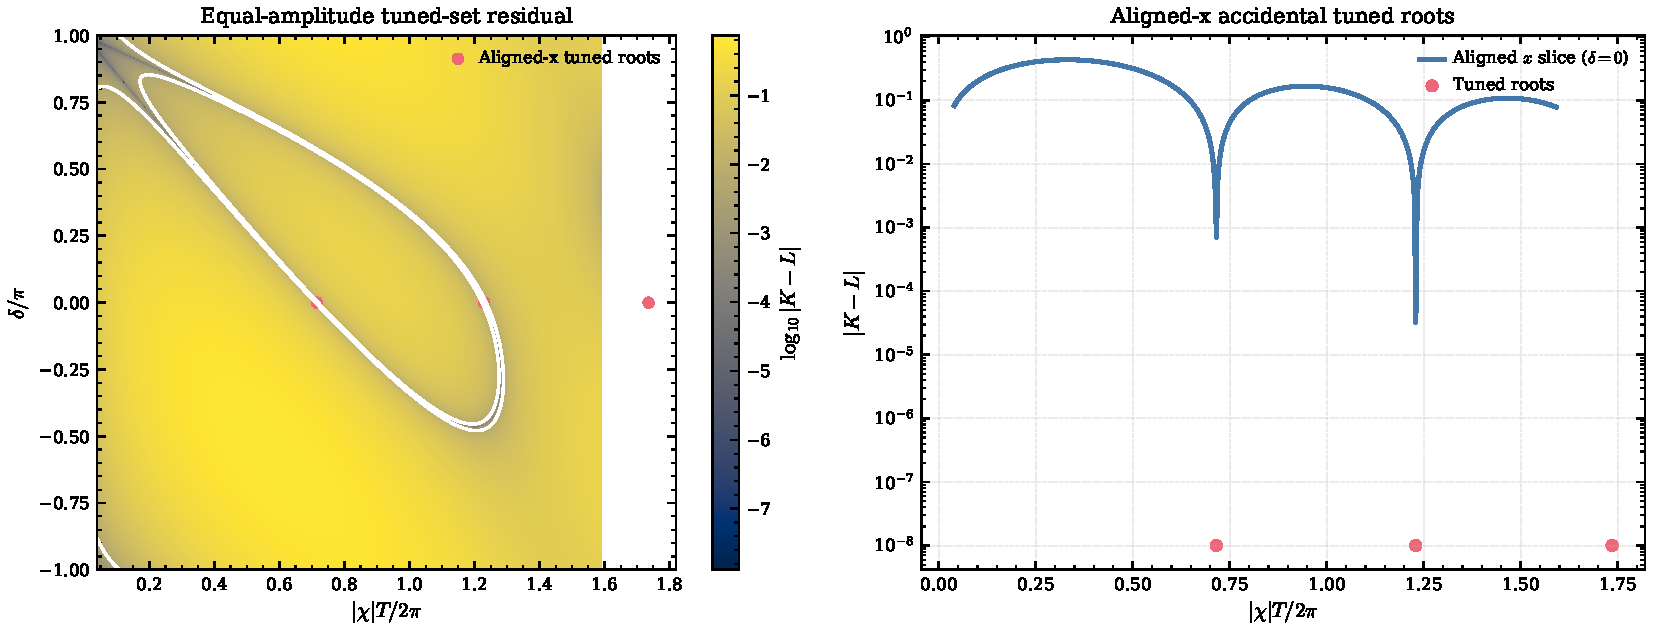
\includegraphics[width=\columnwidth]{../figures/extension_tuned_set_map.pdf}
  \caption{Explicit map of the accidental equal-angle aligned-\(x\) two-block tuned set. The first nontrivial root exists, but it remains a lower-dimensional locus rather than an open region of exact shared-line success.}
  \label{fig:extensiontuned}
\end{figure}

The extension also revisits echoing on the only symmetry-matched family left plausibly favorable: equal-angle aligned-\(x\) targets. The main change is not a reversal of the no-go, but a sharper practical statement. A manifold-aware finite multitone refocusing pulse improves both fidelity and residual \(Z\) relative to the plain strict pulse for the tuned and off-plus checkpoints. At the tuned checkpoint the fidelity rises from \(0.426986\) to \(0.479925\) while the maximum residual \(Z\) drops from \(1.3824\) rad to \(0.7172\) rad. At the off-plus checkpoint the corresponding numbers improve from \(0.517577\) to \(0.537405\) and from \(0.9133\) rad to \(0.6908\) rad. Figure~\ref{fig:extensionecho} shows that this is only partial relief: the best finite echoed checkpoints remain far from ideal and still carry large transverse errors, while the vacuum-calibrated Gaussian echo continues to underperform. The extension therefore narrows the earlier verdict from ``finite echo always fails'' to the more defensible claim that finite echo can help only partially in symmetry-aligned cases and does not rescue generic shared-line selective rotations.

\begin{figure}[tb]
  \centering
  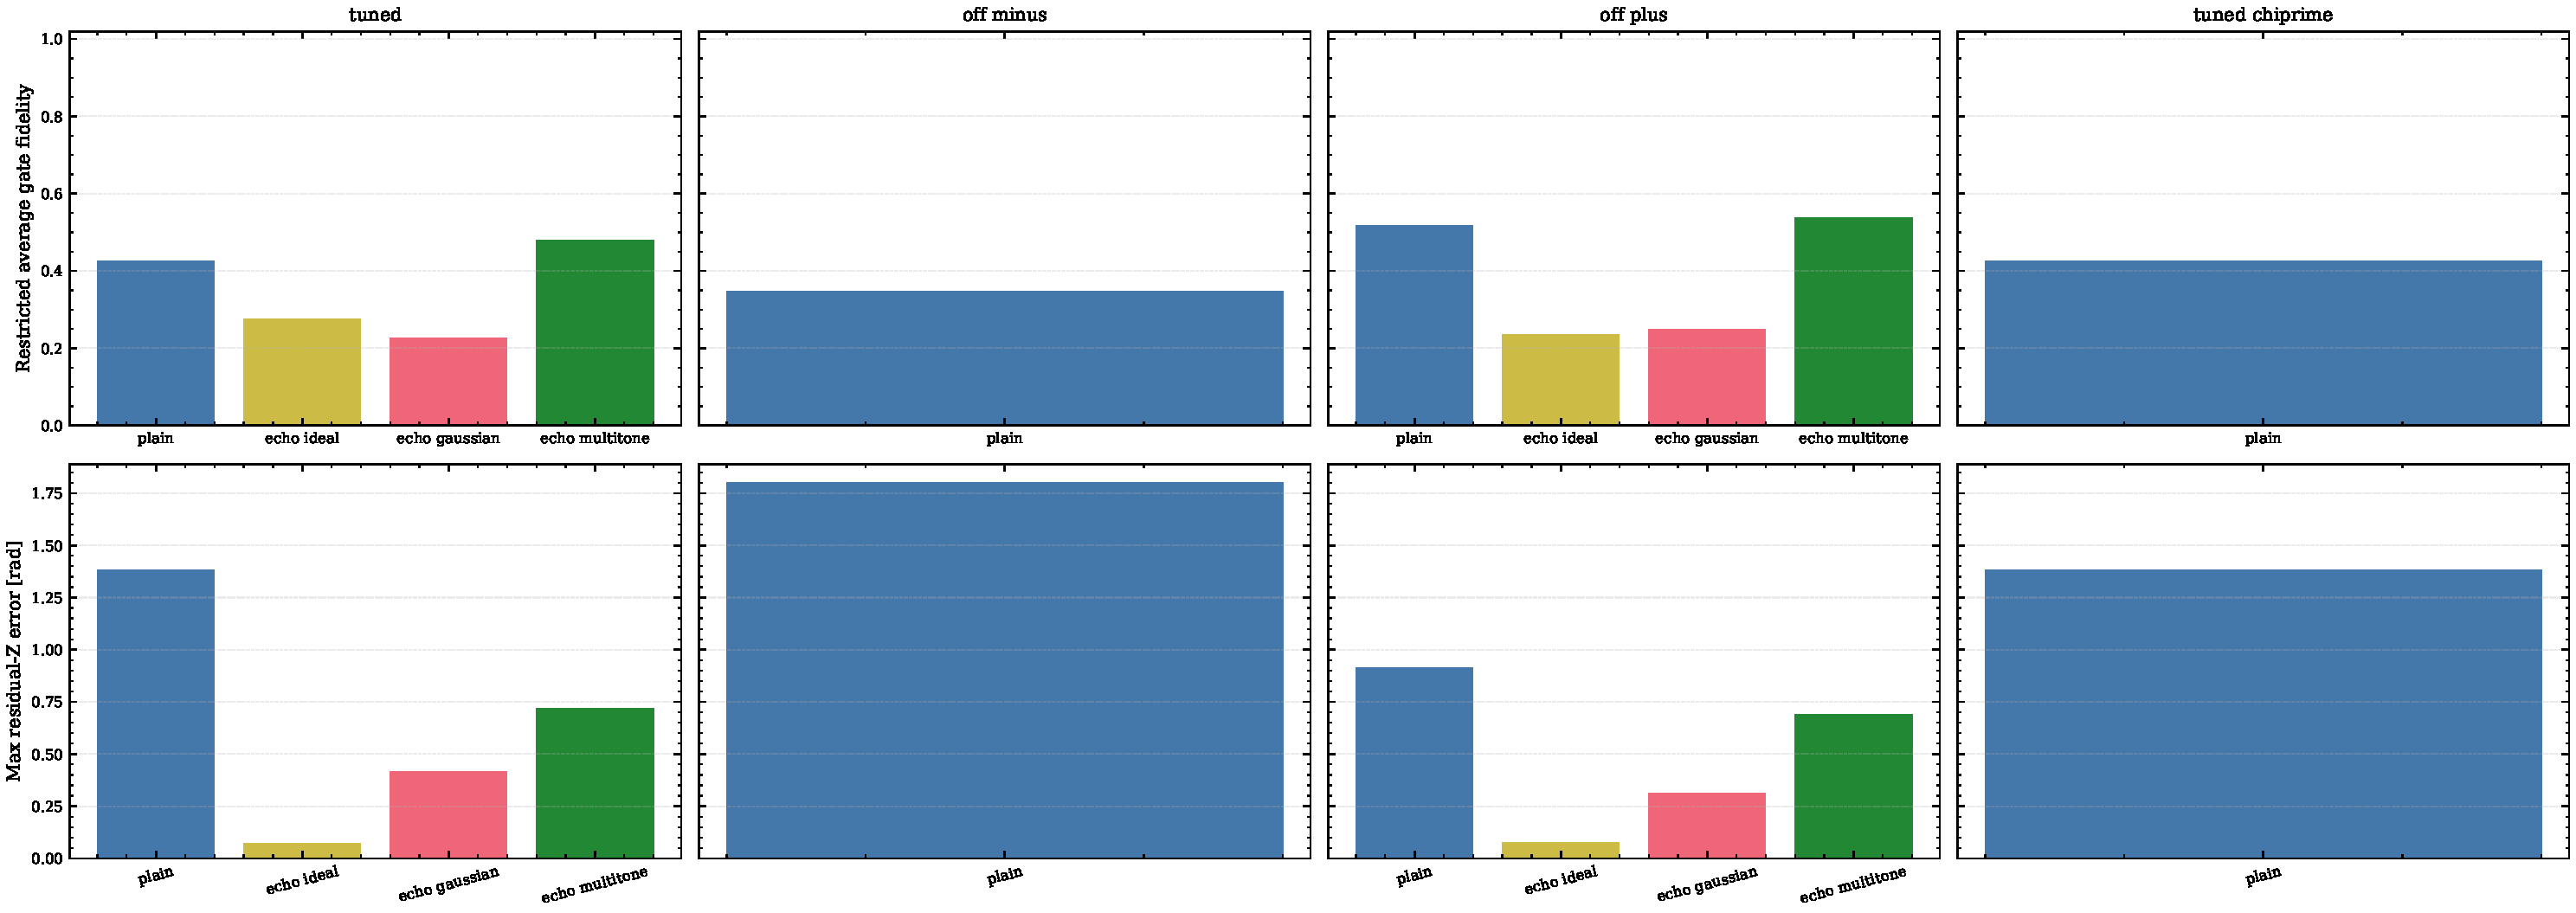
\includegraphics[width=\columnwidth]{../figures/extension_echo_followup_comparison.pdf}
  \caption{Focused echo follow-up on equal-angle aligned-\(x\) checkpoints. A manifold-aware finite refocusing construction can improve both fidelity and residual \(Z\) relative to the plain strict pulse, but the improvement remains partial and far from an ideal gate.}
  \label{fig:extensionecho}
\end{figure}

\section{Validation}
\label{sec:validation}

The baseline production sweep remains validated by the convergence and consistency checks summarized in Appendix~\ref{app:validation}. The extension pass adds three focused checks that are directly tied to the new claims. First, the archived baseline regression reproduced the tracked fidelity and residual-\(Z\) metrics exactly, with zero difference in the stored benchmark quantities. Second, the tuned checkpoint remained internally consistent across timestep changes: at \(dt=\SI{1}{ns},\SI{2}{ns},\SI{4}{ns}\) the restricted average gate fidelity stayed within \(0.4230\) to \(0.4270\), while the maximum residual-\(Z\) error stayed within \(1.3317\) to \(1.3859\) rad. Third, the exact reduced replay continued to match the full shared-line tuned checkpoint at fidelity \(1.0\) for each tested timestep, confirming that the extension conclusions are still rooted in the block-resolved shared-line dynamics rather than in leakage or numerical inconsistency.

\section{Discussion}
\label{sec:discussion}

The extension sharpens rather than overturns the baseline narrative. The tuned-set map shows that the analytical cancellation loci are genuine, but the exact shared-line checkpoints demonstrate that landing on those loci does not open a nearby robust success region. The echo follow-up similarly weakens only the overstrong practical reading, not the underlying obstruction: a symmetry-aware finite echo can improve both fidelity and residual \(Z\) for selected aligned-\(x\) checkpoints, yet the improvement remains modest, comes with longer control sequences, and does not generalize to generic \(XY\) targets because the echo symmetry flips the \(Y\) component. The shared-line no-go is therefore not the consequence of overlooking one clever refocusing convention. It is a structural consequence of trying to realize generic simultaneous blockwise \(XY\) rotations with only shared-line amplitudes and azimuths and no detuning control.

\section{Conclusion}
\label{sec:verdict}

The study prompt asked for four direct answers.

\paragraph*{1. Is exact ideal simultaneous shared-line multitone SQR possible under the physical no-detuning amplitude-plus-azimuth model?}
Not generically. In the controlled dispersive block-resolved regime, the second-order Magnus calculation produces blockwise \(Z\) constraints that are not automatically removable once the transverse target is fixed. Exact shared-line simulations then fail to find any near-unit-fidelity counterexample: the best strict case reaches only \(0.8058\), the mean is \(0.6094\), and even the explicitly mapped tuned aligned-\(x\) checkpoint reaches only \(0.4270\).

\paragraph*{2. Under what assumptions is it impossible?}
The no-go is derived under the shared-line dispersive block-resolved model with simultaneous tones, no artificial per-tone detuning, and the ideal target defined as a direct sum of pure \(XY\) rotations with no block-dependent \(Z\) phase. ``Generically impossible'' means the exact-cancellation set has no open interior in target-and-duration space; only fine-tuned lower-dimensional exceptions remain, and the explicit two-block tuned-set map confirms that those accidental loci do not by themselves restore the full exact gate.

\paragraph*{3. Under what stronger approximation does ideal SQR become achievable?}
If one strengthens the model so that each block retains only its own resonant tone and all spectator tones are dropped exactly, then each block becomes an independently driven qubit and the ideal target is realized by choosing \(\lambda_n=\theta_n/(2T)\) and \(\phi_n=\varphi_n\). That approximation is physically different from the simultaneous shared-line problem because it assumes perfect blockwise decoupling.

\paragraph*{4. Does the echoed multitone sequence rescue the situation exactly, approximately, or only in special regimes?}
Only approximately, and only in special regimes. Ideal instantaneous echoing can suppress some \(Z\)-precession to first order, but it does not preserve the desired gate exactly; for generic \(XY\) targets the transverse axis is mirrored, and even the aligned-\(x\) case retains noncommuting error terms. A symmetry-aware finite multitone echo can improve both fidelity and residual \(Z\) for selected aligned-\(x\) checkpoints, but the best tuned result still stalls at fidelity \(0.4799\) with residual \(Z\) \(0.7172\) rad, so the rescue is partial rather than exact.

\section{Limitations and Future Work}
\label{sec:limitations}

The strongest analytical claim in this report is a controlled no-go inside the block-resolved dispersive model, not an all-regime theorem for arbitrary strong driving. The numerical study is extensive enough to be convincing within that model class, but it still samples a finite target family rather than every conceivable target. The optimizer is also deliberately restricted to the strict amplitude-plus-azimuth ansatz; that is a feature for the present question, not a statement that richer control families are uninteresting.

The extension pass is equally focused rather than exhaustive. Its tuned-set map is constructed for the two-block equal-angle aligned-\(x\) slice because that is the cleanest place where accidental cancellation could plausibly matter, and its echo follow-up is restricted to symmetry-aligned checkpoints and a small family of finite refocusing conventions. Those choices are sufficient to refine the report's practical conclusions, but not to exclude every conceivable partial-echo refinement.

The next steps are therefore clear. First, if the physical goal is exact or near-exact realizability, one should study the minimum extra control resource needed to remove the obstruction cleanly, such as per-tone detuning, explicit \(Z\)-compensation, or genuinely time-segmented control rather than simultaneous shared-line square pulses. Second, if echoed constructions remain of interest, they should be reformulated with manifold-aware refocusing pulses or with a target family aligned to the actual toggling symmetry rather than to a generic \(XY\) axis. Third, the exact reduced blockwise replay and residual-generator diagnostics developed here would be worth upstreaming into the local simulation framework because they make future studies easier to audit.

\appendix

\section{Numerical Details, Validation, and Local Scope Audit}
\label{app:validation}

The strict shared-line sweep consists of \(44\) base cases: two Hamiltonian variants, two deterministic target families, one random target family, addressed windows \(N_{\mathrm{active}}=2,3,4\), and durations \(|\chi|T/2\pi=1,3,5\). Echo was evaluated on the \(24\) deterministic cases with \(N_{\mathrm{active}}\le 3\). The full production sweep required about \(\SI{529}{s}\) on the local workstation.

The representative convergence case is the \(\chi+\chi'\), structured-\(XY\), three-block, \(|\chi|T/2\pi=3\) instance. Re-running that case with a larger optimization budget leaves the restricted average gate fidelity unchanged at \(0.696774\) to six decimal places. Changing the timestep from \(\SI{2}{ns}\) to \(\SI{1}{ns}\) shifts the restricted average gate fidelity only from \(0.696774\) to \(0.697201\), and increasing the transmon truncation from two to three levels changes it from \(0.696774\) to \(0.696958\). Those shifts are small compared with the gap to unit fidelity.

\begin{table}[tb]
  \centering
  \caption{Selected aggregate trends for the strict shared-line model.}
  \label{tab:aggregates}
  \begin{tabular}{@{}lcc@{}}
    \toprule
    Aggregate slice & Mean fidelity & Mean max \(Z\) error (rad) \\
    \midrule
    \(N_{\mathrm{active}}=2\) & 0.6999 & 0.0220 \\
    \(N_{\mathrm{active}}=3\) & 0.5928 & 0.1454 \\
    \(N_{\mathrm{active}}=4\) & 0.5109 & 0.2452 \\
    \(|\chi|T/2\pi=1\) & 0.6500 & 0.0691 \\
    \(|\chi|T/2\pi=3\) & 0.6194 & 0.1295 \\
    \(|\chi|T/2\pi=5\) & 0.5689 & 0.1700 \\
    \bottomrule
  \end{tabular}
\end{table}

\begin{table}[tb]
  \centering
  \small
  \caption{Validation spot checks for the representative structured-\(XY\) three-block case at \(|\chi|T/2\pi=3\).}
  \label{tab:validation}
  \begin{tabular}{@{}lcc@{}}
    \toprule
    Check & Fidelity & Max \(Z\) [rad] \\
    \midrule
    Default settings & 0.696774 & 0.2636 \\
    Smaller timestep & 0.697201 & 0.2355 \\
    Larger timestep & 0.691103 & 0.3151 \\
    Three transmon levels & 0.696958 & 0.2636 \\
    \bottomrule
  \end{tabular}
\end{table}

\begin{table}[tb]
  \centering
  \small
  \caption{Focused extension checkpoints near the aligned-\(x\) tuned locus.}
  \label{tab:extensioncheckpoints}
  \begin{tabular}{@{}lcc@{}}
    \toprule
    Checkpoint & Fidelity & Max \(Z\) [rad] \\
    \midrule
    Tuned & 0.426986 & 1.3824 \\
    Off-minus & 0.346634 & 1.7996 \\
    Off-plus & 0.517577 & 0.9133 \\
    Tuned with \(\chi'\) & 0.426992 & 1.3822 \\
    \bottomrule
  \end{tabular}
\end{table}

\begin{table}[tb]
  \centering
  \small
  \caption{Focused timestep sensitivity for the tuned aligned-\(x\) checkpoint.}
  \label{tab:extensionvalidation}
  \begin{tabular}{@{}lccc@{}}
    \toprule
    \(dt\) [ns] & Fidelity & Max \(Z\) [rad] & Reduced/full \\
    \midrule
    1 & 0.423025 & 1.3859 & 1.0000 \\
    2 & 0.426986 & 1.3824 & 1.0000 \\
    4 & 0.415956 & 1.3317 & 1.0000 \\
    \bottomrule
  \end{tabular}
\end{table}

\begin{figure}[tb]
  \centering
  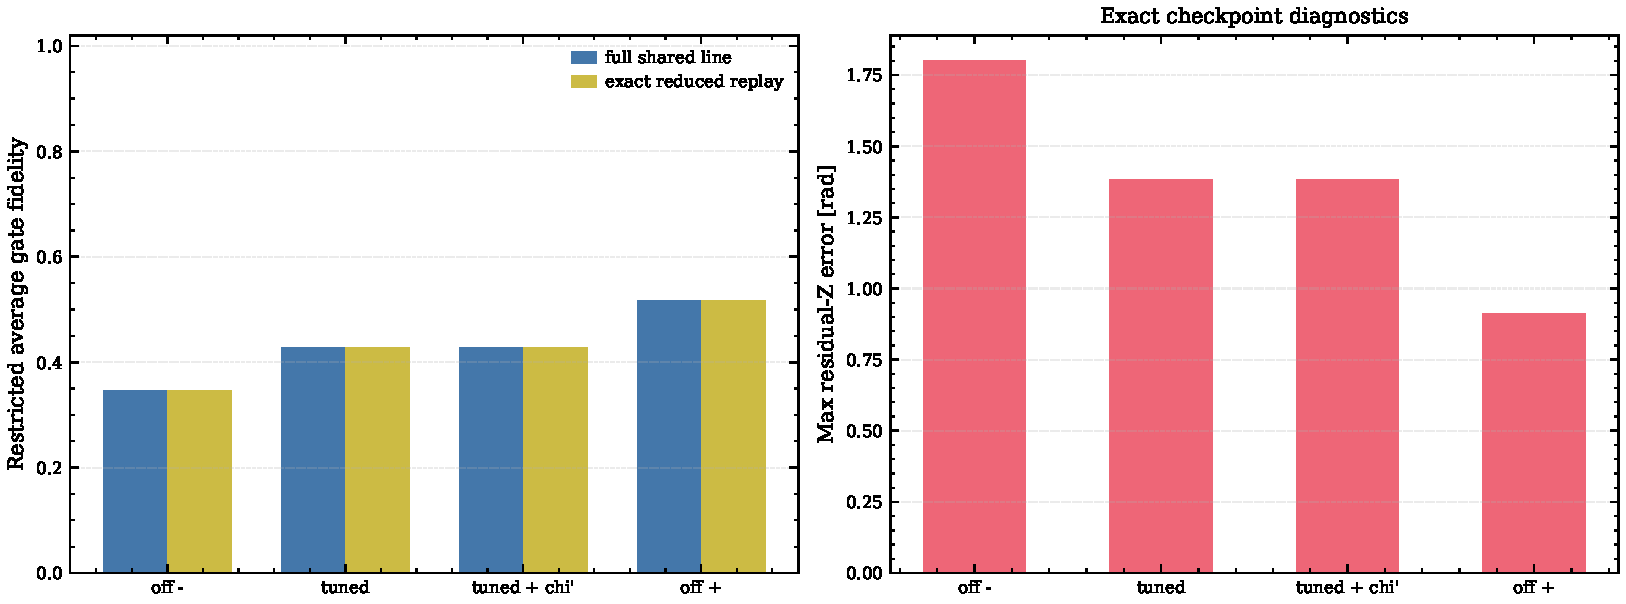
\includegraphics[width=\columnwidth]{../figures/extension_exact_checkpoint_comparison.pdf}
  \caption{Exact shared-line checkpoint comparison around the tuned aligned-\(x\) locus. The analytically tuned point is special, but not optimal, and no nearby checkpoint realizes an ideal shared-line gate.}
  \label{fig:extensioncheckpointsapp}
\end{figure}

The local scope audit was equally important. The nearest earlier studies in this repository did not answer the present question directly because they allowed per-tone frequency corrections, explored richer waveform families, or relaxed the notion of success away from an exact no-detuning ideal-gate test. Those studies are still useful context, but they should not be cited as evidence that the strict shared-line amplitude-plus-azimuth problem is exactly solvable.

The extension pass required about \(\SI{47.6}{s}\) of additional runtime. Its baseline regression reproduced the stored benchmark fidelity and residual-\(Z\) values exactly, and the tuned-case reduced-versus-full comparison remained unity across the tested timestep range. These focused checks justify carrying the extension claims into the main text without reopening the already validated baseline sweep.

\clearpage
\section{Reproducibility}
\label{app:repro}

\begingroup
\sloppy

The machine-readable study outputs are stored under the study data and artifact directories.

\subsection{Baseline summary files}

The main baseline summary files are
\begin{itemize}
  \item \path{study_results.json},
  \item \path{study_results.csv},
  \item \path{study_summary.json},
  \item \path{analytic_summary.json},
  \item \path{validation_summary.json},
  \item \path{prior_audit.json}.
\end{itemize}

\subsection{Extension summary files}

The extension-specific summary files are
\begin{itemize}
  \item \path{extension_tuned_set_map.json},
  \item \path{extension_checkpoint_summary.json},
  \item \path{extension_echo_summary.json},
  \item \path{extension_results.json},
  \item \path{extension_summary.json},
  \item \path{extension_validation_summary.json}.
\end{itemize}

\subsection{Stored case artifacts}

\begin{description}
  \item[Restricted operators.] {\raggedright Stored under \path{artifacts/cases/}. Extension checkpoints use the \path{extension_} filename prefix.\par}
  \item[Compiled waveforms.] {\raggedright Stored under \path{artifacts/waveforms/}.\par}
  \item[Extension figures.] {\raggedright Archived in both \path{.pdf} and \path{.png} formats in the figure directory.\par}
  \item[Notebook.] {\raggedright Stored at \path{scripts/reproducibility_notebook.ipynb}.\par}
\end{description}

\subsection{Reproduction procedure}

The shortest complete reproduction path is:
\begin{description}
  \item[Baseline generation.] {\raggedright Run \path{scripts/run_study.py}. This regenerates the baseline shared-line, reduced, decoupled, and echoed results.\par}
  \item[Baseline validation.] {\raggedright Run \path{scripts/validate_results.py}. This reproduces the baseline convergence and sanity summary.\par}
  \item[Extension generation.] {\raggedright Run \path{scripts/run_extension_study.py}. This rebuilds the tuned-set map, focused checkpoints, and aligned-echo follow-up.\par}
  \item[Extension validation.] {\raggedright Run \path{scripts/validate_extension.py}. This reproduces the focused extension validation package.\par}
  \item[Notebook refresh.] {\raggedright Rebuild \path{scripts/reproducibility_notebook.ipynb} with \path{scripts/build_reproducibility_notebook.py} whenever the saved artifacts change.\par}
  \item[Report build.] {\raggedright Compile the report from the report directory after the data products are in place.\par}
\end{description}

\endgroup

\bibliographystyle{apsrev4-2}
\bibliography{references}

\end{document}
